\subsection{平面的基本性质}\label{subsec:1-2}

在生产与生活中,人们经过长期的观察与实践,总结出关于平面的三个基本性质。
我们把它们当作公理,作为进一步推理的基础。

\begin{gongli}[公理1][gl:pm-1]% gl: 公理;  pm: 平面
    如果一条直线上的两点在一个平面内,那么这条直线上所有的点都在这个平面内
\end{gongli}(图 \ref{fig:ltjh-1-3})。

\begin{figure}[htbp]
    \centering
    \begin{minipage}[b]{4cm}
        \centering
        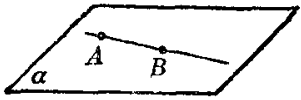
\includegraphics[width=4cm]{../pic/ltjh-ch1-03.png}
        \caption{}\label{fig:ltjh-1-3}
    \end{minipage}
    \qquad
    \begin{minipage}[b]{4cm}
        \centering
        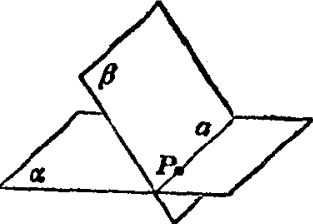
\includegraphics[width=4cm]{../pic/ltjh-ch1-04.png}
        \caption{}\label{fig:ltjh-1-4}
    \end{minipage}
    \qquad
    \begin{minipage}[b]{4cm}
        \centering
        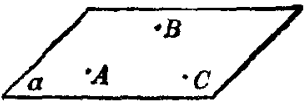
\includegraphics[width=4cm]{../pic/ltjh-ch1-05.png}
        \caption{}\label{fig:ltjh-1-5}
    \end{minipage}
\end{figure}


这时我们说直线在平面内,或者说平面经过直线。

例如,把一根直尺边缘上的任意两点放在平的桌面上,可以看到直尺边缘就落在桌面上。

点 $A$ 在直线 $a$ 上,记作 $A \in a$;
点 $A$ 在直线 $a$ 外,记作 $A \not \in a$;
点 $A$ 在平面 $\alpha$ 内,记作 $A \in \alpha$,
点 $A$ 在平面 $\alpha$ 外,记作 $A \not \in \alpha$;
直线 $a$ 在平面 $\alpha$ 内,记作 $a \subset\alpha$。

\begin{gongli}[公理2][gl:pm-2]
    如果两个平面有一个公共点,那么它们有且只有一条通过这个点的公共直线
\end{gongli}(图 \ref{fig:ltjh-1-4})。


例如,教室内相邻的墙面,在墙角处交于一个点,它们就交于过这个点的一条直线。

如果两个平面 $\alpha$ 和 $\beta$ 有一条公共直线 $a$,就说平面 $\alpha$ 和 $\beta$ 相交,
交线是 $a$,记作 $\alpha \cap \beta = a$。

\begin{gongli}[公理3][gl:pm-3]
    经过不在同一条直线上的三点,有且只有一个平面
\end{gongli}(图 \ref{fig:ltjh-1-5})。

例如,一扇门用两个合页和一把锁就可以固定了。

过 $A$、$B$、$C$ 三点的平面又可记作“平面 $ABC$”。

根据上述公理,可以得出下面的推论:

\begin{tuilun}[推论1][tl:pm-1] % tl: 推论
    经过一条直线和这条直线外的一点,有且只有一个平面
\end{tuilun}(图 \ref{fig:ltjh-1-6} 甲)。

\begin{figure}[htbp]
    \centering
    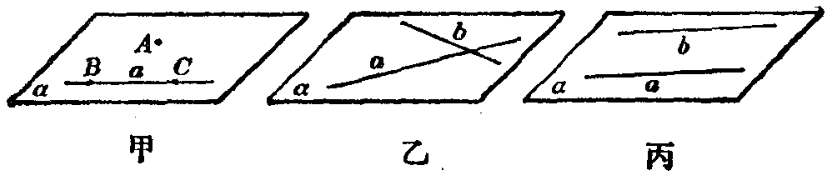
\includegraphics[width=10cm]{../pic/ltjh-ch1-06.png}
    \caption{}\label{fig:ltjh-1-6}
\end{figure}

$A$ 是直线 $a$ 外的一点,在 $a$ 上任取两点 $B$、$C$。
根据\nameref{gl:pm-3},经过不共线的三点 $A$、$B$、$C$ 有一个平面 $\alpha$。
因为点 $B$、$C$ 都在平面 $\alpha$ 内,所以根据\nameref{gl:pm-1},直线 $a$ 在平面 $\alpha$ 内。
即平面 $\alpha$ 是经过直线 $a$ 和点 $A$ 的平面。

因为点 $B$、$C$ 在直线 $a$ 上,所以经过直线 $a$ 和点 $A$ 的平面一定经过点 $A$、$B$、$C$。
又根据\nameref{gl:pm-3} 经过不共线的三点 $A$、$B$、$C$ 的平面只有一个,
所以经过直线 $a$ 和点 $A$ 的平面只有一个。

类似地,可以得出下面两个推论:

\begin{tuilun}[推论2][tl:pm-2]
    经过两条相交直线,有且只有一个平面
\end{tuilun}(图 \ref{fig:ltjh-1-6} 乙)。

\begin{tuilun}[推论3][tl:pm-3]
    经过两条平行直线,有且只有一个平面
\end{tuilun}(图 \ref{fig:ltjh-1-6} 丙)。

“有且只有一个平面”,我们也说“确定一个平面”。

\zhuyi 在立体几何里,平面几何中的定义、公理、定理等,对于同一个平面内的图形仍然成立。


\liti[0] 两两相交且不过同一个点的三条直线必在同一个平面内。

已知:直线 $AB$、$BC$、$CA$ 两两相交,交点分别为 $A$、$B$、$C$(图 \ref{fig:ltjh-1-7})。

\begin{wrapfigure}[5]{r}{7cm}
    \centering
    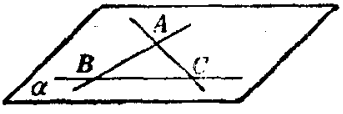
\includegraphics[width=4cm]{../pic/ltjh-ch1-07.png}
    \caption{}\label{fig:ltjh-1-7}
\end{wrapfigure}

求证:直线 $AB$、$BC$、$CA$ 共面 \footnotemark 。
\footnotetext{空间的几个点和几条直线,如果都在同一个平面内,可以简单地说它们“共面”,否则说它们“不共面”。}

\zhengming $\because$ \quad 直线 $AB$ 和 $AC$ 相交于点 $A$,

$\therefore$ \quad 直线 $AB$ 和 $AC$ 确定一个平面 $\alpha$ (\nameref{tl:pm-2})。

$\because$ \quad $B \in AB$, $C \in AC$,

$\therefore$ \quad $B \in \alpha$, $C \in \alpha$。

$\therefore$ \quad $BC \subset \alpha$ (\nameref{gl:pm-1})。

因此,直线 $AB$、$BC$、$CA$ 都在平面 $\alpha$ 内,即它们共面。


\begin{lianxi}

\xiaoti{填空:}
\begin{xiaoxiaotis}

    \xxt{\xhx[3cm] 的三点确定一个平面;}

    \xxt{两条 \xhx[1.5cm] 或 \xhx[1.5cm] 直线确定一个平面;}

    \xxt{有一个公共点的两个平面相交于 \xhx[2cm] 一条直线。}

\end{xiaoxiaotis}


\xiaoti{用符号表示下列语句:}
\begin{xiaoxiaotis}

    \xxt{点 $A$ 在平面 $\alpha$ 内,但在平面 $\beta$ 外;}

    \xxt{直线 $a$ 经过平面 $\alpha$ 外一点 $M$;}

    \xxt{直线 $a$ 和 $b$ 相交于平面 $\alpha$ 内一点 $M$;}

    \xxt{直线 $a$ 在平面 $\alpha$ 内,又在平面 $\beta$ 内,平面 $\alpha$ 和 $\beta$ 相交于直线 $a$。}

\end{xiaoxiaotis}


\xiaoti{将下列命题改写成语言叙述,判断它们是否正确,并说明理由。}
\begin{xiaoxiaotis}

    \xxt{当 $A \in \alpha$, $B \not \in \alpha$ 时,线段 $AB \subset \alpha$;}

    \xxt{$\left.\begin{aligned}
        & A \in \alpha \\
        & B \in \alpha \\
        & C \in AB
    \end{aligned}\right\} \tuichu C \in \alpha \juhao$}

\end{xiaoxiaotis}

\end{lianxi}
